\def\QRCODE{TB_IPR_TUT.IMG.convexhull_matlabqrcode.png}
\def\QRPAGE{http://www.iptutorials.science/tree/master/TB_IPR/TUT.IMG.convexhull/matlab}
\mcorrectionsection{Matlab correction}

\subsection{Graham scan algorithm}
The convex hull function starts by giving the points as parameters:
\begin{matlab}
function Q=conv_hull(PointsOri)
% PointsOri: original point set
\end{matlab}

This function follows the stated algorithm (Graham Scan).
\begin{itemize}
 \item find lowest y-axis point
 \item sort points by their angle
 \item proceed in this order and check left or right turn
\end{itemize}

For convex hull and other computational geometry algorithms, robustness must be handled with special care. Floating points operations may be really tricky and the following code is not ensured to work for all cases.


\begin{matlab}
% very naive precision handling
Points=round(PointsOri.*1000)/1000;
\end{matlab}

The first step is to get the starting point.
\begin{matlab}
% get points with minimal y-coordinate
PP = sortrows(Points, [2 1]);
P = PP(1,:);
\end{matlab}

Then, the points are sorted by the opposite of the cosine of the angle, because cosine is decreasing on the interval $[0;\pi]$. This step has complexity $O(n\log n)$.
\begin{matlab}
Points=PP(2:end, :);

% sort by cosinus of angle
adj_side=Points(:,1)-P(1);
opp_side=Points(:,2)-P(2);
hypothenuse=sqrt(adj_side.^2+opp_side.^2);
cosinus=adj_side./hypothenuse;
[~,ind]=sort(-cosinus); % cos is decreasing
Points=[P;Points(ind,:);P];
\end{matlab}

Finally, the sorted points allow to construct the convex hull by testing the orientation of the turn of the hull (see Fig.\ref{fig:matlab:convexhull:pause}). 
\begin{matlab}
% compute convex hull in this order
Q=[];
Q=push(Q,Points(1,:));
Q=push(Q,Points(2,:));
for i=3:size(Points,1)
    while (length(Q)>=2 && CrossProduct(Q,Points(i,:)) < 0)
        Q=pop(Q);
    end
    Q=push(Q,Points(i,:));
end
\end{matlab}

\begin{figure}[htbp]
 \centering
 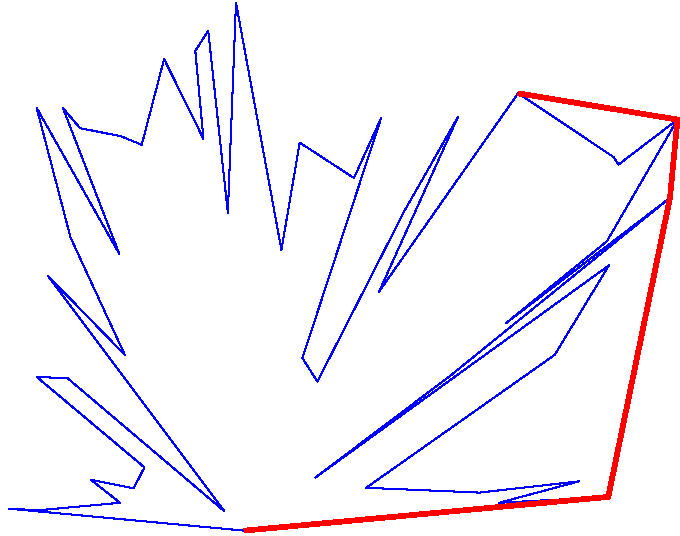
\includegraphics[width=.45\linewidth]{chull_50_pause.pdf}
 \caption{Graham scan illustration while constructing the convex hull.}
 \label{fig:matlab:convexhull:pause}
\end{figure}

\subsection{Useful functions}
These 3 functions are used to push and pop a point in a list, and to compute the cross-product. 

\begin{mcomment}
\begin{mremark}
 The \matlabregistered{} function \minline{cross} could have been used.
\end{mremark}
\end{mcomment}


\begin{matlab}    
function Z=push(Q,point)
    % point into a list
    Z=[Q;point];
end
\end{matlab}
\begin{matlab}
function Z=pop(Q)
    % pop last element
    Z=Q(1:end-1,:);
end
\end{matlab}

This cross-product function first extract the last two points of the hull, and check if there is a left-turn or a right-turn to go to the point $p_3$.
\begin{matlab}
function p=CrossProduct(Q, p3)
    % cross product 
    % Q  : list of points (hull)
    % p3 : point
    p1=Q(end-1,:);
    p2=Q(end,:);
    p=(p2(1) - p1(1))*(p3(2) - p1(2)) - (p3(1) - p1(1))*(p2(2) - p1(2));
end
\end{matlab}


\subsection{Simple tests}
For 5 points:
\begin{matlab}
Points=[1  1  3 4 3;
        2 -4 -4 1 0];
Points=Points';

plot(Points(:,1),Points(:,2),'*')
axis equal
Q=conv_hull(Points);
hold on;
plot(Q(:,1),Q(:,2),'r')

\end{matlab}

For a few random points:
\begin{matlab}
n=50;
Points2=rand(n,2);

figure
plot(Points2(:,1),Points2(:,2),'*')
axis equal
Q=conv_hull(Points2);
hold on;
plot(Q(:,1),Q(:,2),'r')
\end{matlab}

The results are illustrated in Fig.\ref{fig:matlab:convexhull:res}.

\begin{figure}[htbp]
\centering

\subfloat[Convex points of 5 points.]{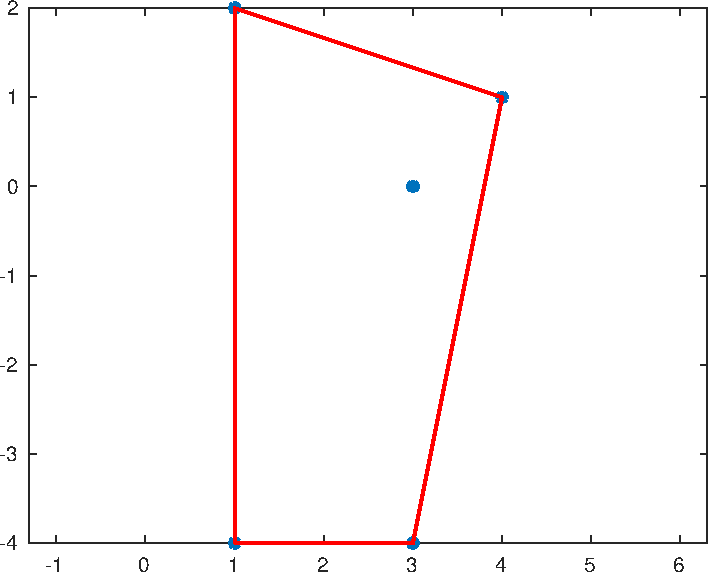
\includegraphics[width=.45\linewidth]{chull_5.pdf}}\hfill
\subfloat[Convex hull of 50 random points.]{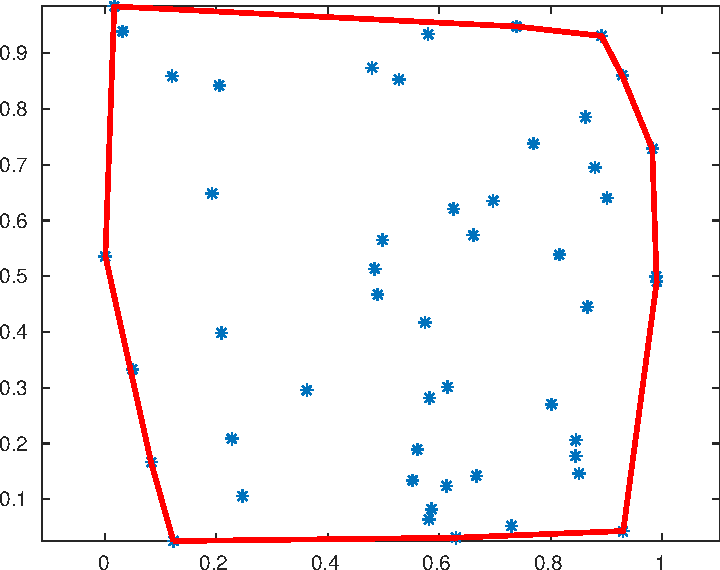
\includegraphics[width=.45\linewidth]{chull_50.pdf}}

\caption{Illustration of the convex hull computation.}
\label{fig:matlab:convexhull:res}
\end{figure}


